\section{Setting}
\label{sec:setting}


This paper presents \sysnameF to augment encrypted deduplication by {\em proactively detecting the learning-content attack} in a client-side {\em trusted execution environment (TEE)}, so as to fully defeat against the malicious client.

\paragraph{Trusted execution.} We build on {\em Intel Software Guarded Extensions (SGX)} \cite{sgx} to realize the TEE, since SGX is widely supported by today's commodity computers. In addition to SGX, our design (\S\ref{sec:design}) can be extended to other trusted computing technologies \cite{amd-sev, pinto19} that support TEE.

SGX extends Intel CPU with a set of security-related instructions to realize a TEE. It allocates an {\em enclave} in a hardware-guarded memory region (called {\em enclave page cache (EPC)}), in order to host (in-enclave) contents with confidentiality and integrity guarantees. After an enclave is created, SGX provides {\em remote attestation} to authenticate the enclave via a remote entity (e.g., the cloud), as well as {\em secret provisioning} to share a secret key between the (authenticated) encalve and the cloud. Also, SGX provides two interfaces for the interaction between the enclave and  unprotected memory. A program can enter the enclave to execute in-enclave functions via {\em enclave calls (ECalls)}. Within an ECall, it can temporarily exit the enclave and call untrusted functions in unprotected memory via {\em outside calls (OCalls)}.



\paragraph{Deployment scenario.} Figure~\ref{fig:model} presents the scenario of encrypted deduplication (\S\ref{sub:basics}). To deploy \sysnameF, we first compile the enclave code into a shared object \cite{sgx}, and distribute the shared object along with a signature for integrity verification to each client. The cloud  hosts the shared object to validate the enclave of each client.
Specifically, the client initializes \sysnameF to create the corresponding enclave by loading the shared object, and the cloud authenticates each enclave via remote attestation \cite{sgx} to ensure that the correct code is loaded into the enclave.

In the upload procedure, \sysnameF processes plaintext chunks (that are generated by the client), and computes corresponding ciphertext chunks and fingerprints for source-based deduplication. A non-compromised client only transfers non-duplicate ciphertext chunks to the cloud, while \sysnameF reports a malicious client if the client is caught to launch the learning-content attack.

\begin{figure}
  \centering
  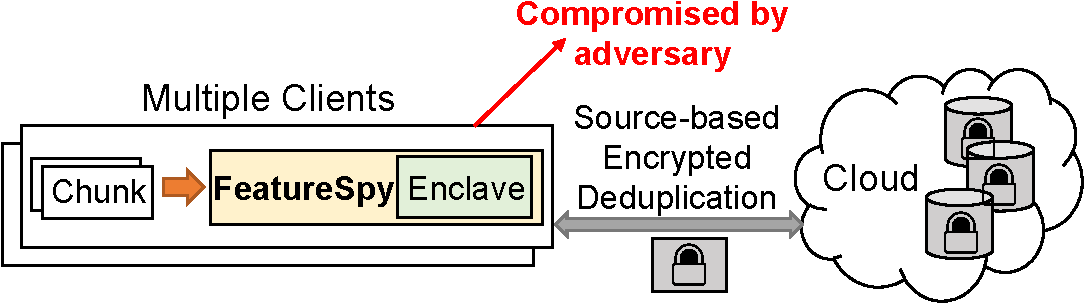
\includegraphics[width=3.25in]{pic/featurespy/deployment.pdf}
  \vspace{-6pt}
  \caption{Deployment of \sysnameF.}
  \label{fig:model}
  \vspace{-6pt}
\end{figure}


% \paragraph{Challenges of design with SGX.} Although SGX supports plenty of security features, it is necessary to judiciously make design decisions, which affect the security  and performance of \sysnameF. Specifically, the {\em trusted computing base (TCB)} of an SGX enclave includes the Intel CPU, in-enclave code and data, and (enclave) interface function calls. A large TCB facilitates design, yet increasing security risks since a lot of interface calls may behave in unpredictable ways \cite{lie05}.

% Also, when the in-enclave content has a larger size than EPC (whose size is limited by 128\,MiB), SGX encrypts unused EPC pages and evicts them to unprotected memory, leading to high {\em EPC paging overhead} \cite{dinhngoc19}. Although the latest version of SGX supports a larger EPC size up to 1\,TiB \cite{sgx2}, it loses the integrity tree protection \cite{feng21}.

% Furthermore, both ECalls and OCalls add  context-switch overhead \cite{arnautov16}. The code that is just running in the enclave (i.e., without accessing unprotected memory) even incurs performance drop over that is running in unprotected memory \cite{harnik18}.

%



% The foremost issue of designing \sysnameF is to decide detecting the learning-content attack in either the cloud or the client side.
% A cloud-side detection system can view the uploads of all clients, and monitor their behaviors. However, the uploaded contents include chunk fingerprints that are random by nature, and non-duplicate ciphertext chunks that form just a partial view of each client's behavior. Such information is insufficient to reason about the learning-content attack.

% Thus, we choose to design \sysnameF for client-side deployment, while running the detection process in a {\em shielded environment} to protect against a malicious client that  may tamper the system to escape detection (\S\ref{sub:threat}).



% \subsection{Intel SGX}
% \label{sub:sgx}

% \paragraph{SGX basics.} SGX extends Intel CPU with a set of security-related instructions to realize a shielded execution environment. It allocates an {\em enclave} in a hardware-guarded memory region (called {\em enclave page cache (EPC)}), in order to host (in-enclave) contents with confidentiality and integrity guarantees. After an enclave is initialized, SGX provides {\em remote attestation} to authenticate the enclave via a remote entity (e.g., the cloud), as well as {\em secret provisioning} to share a secret key between the (authenticated) encalve and the cloud. Also, SGX provides two interfaces for the interaction between the enclave and  unprotected memory. A program can enter the enclave to execute in-enclave functions via {\em enclave calls (ECalls)}. Within an ECall, it can temporarily exist the enclave and call untrusted functions in unprotected memory via {\em outside calls (OCalls)}.



% \paragraph{Challenges of design with SGX.} Although SGX supports plenty of security features, it is necessary to judiciously make design decisions, which affect the security  and performance of \sysnameF. Specifically, the {\em trusted computing base (TCB)} of an SGX enclave includes the Intel CPU, in-enclave code and data, and (enclave) interface function calls. A large TCB facilitates design, yet increasing security risks since a lot of interface calls may behave in unpredictable ways \cite{lie05}.

% Also, when the in-enclave content has a larger size than EPC (whose size is limited by 128\,MiB), SGX encrypts unused EPC pages and evicts them to unprotected memory, leading to high {\em EPC paging overhead} \cite{dinhngoc19}. Although the latest version of SGX supports a larger EPC size up to 1\,TiB \cite{sgx2}, it loses the integrity tree protection \cite{feng21}.

% Furthermore, both ECalls and OCalls add  context-switch overhead \cite{arnautov16}. The code that is just running in the enclave (i.e., without accessing unprotected memory) even incurs performance drop over that is running in unprotected memory \cite{harnik18}.



\paragraph{Threat model.} Our major security goal is to enhance encrypted deduplication (\S\ref{sub:basics}) with security against a {\em malicious} client. Like encrypted deduplication \cite{bellare13a}, we consider a compromised cloud that aims to eavesdrop the original content from any stored ciphertext chunk. In addition, we consider a malicious client that aims to learn the original plaintext chunks of other non-compromised clients. Specifically, the malicious client can access its compromised  plaintext chunks and keys, and arbitrarily fake new plaintext chunks to launch the learning-content attack (\S\ref{sub:basics}). Also, it can tamper with the  contents and operations in unprotected memory, in order to escape the capture of \sysnameF.
Our threat model makes the following assumptions.
\begin{itemize}[leftmargin=*]
\item The communication channel between each client and the cloud is protected by SSL/TLS against eavesdropping.
\item
  The SGX enclave is trusted and authenticated (e.g., via remote attestation when it is first bootstrapped), so as to honestly perform attack detection against tampering. Also, like the previous works \cite{shinde20, ren21}, the SGX enclave preserves confidentiality for only a cryptographic key (i.e., the proof key in \S\ref{sec:implementation}) rather than all in-enclave contents; this is important in light of the side-channel attacks against SGX (e.g., see \cite{fei21} for a survey).

%   trusted, and authenticated by remote attestation (\S\ref{sub:sgx}) when it is first bootstrapped.
% It assumes the confidentiality of SGX only in one lemma, i.e., the secrecy of a cryptographic key. This is an important design choice in light of the side-channels
%  Although previous studies  report the security vulnerabilities of SGX, they are orthogonal
 % to \sysnameF, which can be enchanced with  future improvements of SGX.
% \item \sysnameF augments PoW \cite{halevi11, ren21}, and naturally addresses the threat that uses a fingerprint to obtain the ownership of the corresponding chunk (\S\ref{sub:basics}).
\item A malicious cloud may corrupt outsourced data to compromise integrity. \sysnameF does not address the threat, yet it is compatible with {\em proof data prosession (PDP)} \cite{ateniese07} and {\em proof of retrievability (PoR)} \cite{juels07} to perfrom periodically integrity verification of outsourced data, as well as fault-tolerant storage to recover data from corruption \cite{li15}.
\end{itemize}
